\documentclass[sigconf,nonacm]{acmart}
\settopmatter{printacmref=false}
\setcopyright{none}
\renewcommand\footnotetextcopyrightpermission[1]{}

\usepackage{graphicx}
\graphicspath{{../figures/}}
\usepackage{booktabs}
\usepackage{stfloats}

% ─── METADATA ────────────────────────────────────────────────────────────────
\title{Fourier Neural Operators for 2D Navier--Stokes: A Comparison with U-Net}

\author{Ian Havill}
\affiliation{\institution{Occidental College}\city{Los Angeles}\state{CA}\country{USA}}
\email{havill@oxy.edu}

\author{Hugh Baldwin}
\affiliation{\institution{Occidental College}\city{Los Angeles}\state{CA}\country{USA}}

\author{Aaron Chen}
\affiliation{\institution{Occidental College}\city{Los Angeles}\state{CA}\country{USA}}

\date{May 2026}


% ─── DOCUMENT ────────────────────────────────────────────────────────────────
\begin{document}

\begin{abstract}
We compare the Fourier Neural Operator (FNO) \cite{li2021fno} against a standard
U-Net \cite{ronneberger2015unet} on the task of predicting the one-step time
evolution of 2D incompressible Navier--Stokes equations.
Both models are trained on 10{,}000 vorticity field pairs at 128$\times$128
resolution drawn from the neuraloperator Zenodo dataset \cite{zenodo2024}.
FNO achieves a test relative-$L^2$ error of 0.0348 with 4.7M parameters,
outperforming U-Net (relative-$L^2$ = 0.1029, 31M parameters) by a factor of
roughly $3\times$ while using $6.6\times$ fewer parameters and running $2.2\times$
faster.
In zero-shot super-resolution experiments---where both models are evaluated at
resolutions never seen during training---FNO's error remains flat (0.019 across
64, 128, and 256 grid points per side), while U-Net's error degrades by
$4$--$6\times$ at unseen resolutions.
These results illustrate how architectures that encode physical structure in the
frequency domain can outperform generic convolutional baselines on PDE surrogate
tasks.
\end{abstract}

\maketitle

% ─── INTRODUCTION ────────────────────────────────────────────────────────────
\section{Introduction}
\label{sec:intro}

Simulating fluid dynamics is a central problem in science and engineering, with
applications ranging from weather forecasting and aircraft design to biomedical
flow modelling.
The governing equations---the Navier--Stokes (NS) equations---are well understood
mathematically, but numerically solving them is expensive: a typical high-fidelity
simulation on a fine spatial grid requires minutes to hours on powerful hardware,
and must be repeated from scratch for each new set of initial conditions.

A natural alternative is to \emph{learn} the simulation from data.
Rather than solving the PDE numerically each time, one trains a neural network to
approximate the solution operator $\mathcal{G}: u(t) \mapsto u(t + \Delta t)$
directly, and then evaluates it at inference time.
If this operator can be learned efficiently, inference is a single forward pass
taking milliseconds.

The key challenge is that the solution operator maps \emph{functions} (vorticity
fields) to functions, not fixed-length vectors.
Standard convolutional networks (CNNs) are tied to the resolution they were
trained at and carry no principled notion of function-space generalization.
Li et al.\ \cite{li2021fno} introduced the \emph{Fourier Neural Operator} (FNO),
which operates in frequency space and is, by design, resolution-independent.

In this work we benchmark FNO against a U-Net \cite{ronneberger2015unet}---a
widely used CNN architecture---on the 2D Kolmogorov-forced Navier--Stokes
problem.
We evaluate both models on (1) standard accuracy and inference speed, and (2)
zero-shot super-resolution: the ability to generalize to grid resolutions the
model was never trained on.

% ─── BACKGROUND ──────────────────────────────────────────────────────────────
\section{Background}
\label{sec:background}

\subsection{2D Navier--Stokes Equations}

We consider the 2D incompressible Navier--Stokes equations in vorticity form on
the unit torus $[0,1]^2$:
\begin{align}
  \frac{\partial \omega}{\partial t} + (\mathbf{u} \cdot \nabla)\omega
    &= \nu\,\nabla^2 \omega + f, \label{eq:ns}\\
  \omega &= \nabla \times \mathbf{u}, \quad \nabla \cdot \mathbf{u} = 0.
\end{align}
Here $\omega$ is the vorticity scalar, $\mathbf{u}$ is the velocity field, $\nu$
is kinematic viscosity, and $f$ is an external body force.
We use the Kolmogorov forcing $f(x,y) = \sin(4\pi y)$, which injects energy at
low wavenumbers and drives the system into a turbulent regime.
With $\nu = 10^{-4}$ the Reynolds number is $Re = 10{,}000$, placing the flow
firmly in the turbulent regime.

The task is to learn the discrete time-stepping operator: given $\omega$ at time
$t$, predict $\omega$ at time $t + \Delta t$.

\subsection{Fourier Neural Operator}

A classical integral operator kernel $\mathcal{K}$ applied to a function $v$ can
be written as a convolution:
\begin{equation}
  (\mathcal{K}v)(x) = \int_D \kappa(x - y)\, v(y)\,dy,
\end{equation}
which in Fourier space becomes a pointwise multiplication:
\begin{equation}
  (\mathcal{K}v)(x) = \mathcal{F}^{-1}\!\bigl(R_\phi \cdot \mathcal{F}(v)\bigr)(x),
\end{equation}
where $R_\phi$ is a tensor of learnable complex weights.
The FNO implements this as a layer that (i) applies a 2D FFT, (ii) truncates to
the lowest $k$ Fourier modes, (iii) multiplies by learned complex weights, and
(iv) applies the inverse FFT.
A residual 1$\times$1 convolution is added in parallel to capture local structure.

Because the operation is defined in frequency space, it is resolution-agnostic:
the same learned weights can be applied to inputs at any spatial resolution.

\subsection{U-Net}

The U-Net \cite{ronneberger2015unet} is a convolutional encoder--decoder
architecture.
An encoder successively halves the spatial resolution while doubling the channel
count; a symmetric decoder upsamples back to the original resolution.
Skip connections concatenate encoder feature maps into the corresponding decoder
stages, preserving fine spatial detail.
All operations are local spatial convolutions, so U-Net has no intrinsic mechanism
for generalizing across resolutions.

% ─── DATASET ─────────────────────────────────────────────────────────────────
\section{Dataset}
\label{sec:dataset}

We use the \texttt{nsforcing\_128} dataset from the neuraloperator Zenodo
archive \cite{zenodo2024} (doi:10.5281/zenodo.12825163).
The dataset consists of 12{,}000 pairs $(x, y)$ where each is a
$128\times 128$ vorticity field: $x = \omega(t)$ and $y = \omega(t + \Delta t)$.
We use 10{,}000 pairs for training and 2{,}000 for evaluation.
Data is stored as PyTorch \texttt{.pt} tensors.

Input vorticity fields have low amplitude (std $\approx 0.15$, range $[-0.76,
0.82]$), while target fields are more energetic (std $\approx 0.71$, range
$[-3.49, 3.93]$), reflecting the turbulent energy cascade over one timestep.
The per-sample standard deviations are nearly linearly correlated, confirming
the dataset is internally consistent.
Figure~\ref{fig:sample_pairs} shows representative input--target pairs.

\begin{figure}[t]
  \centering
  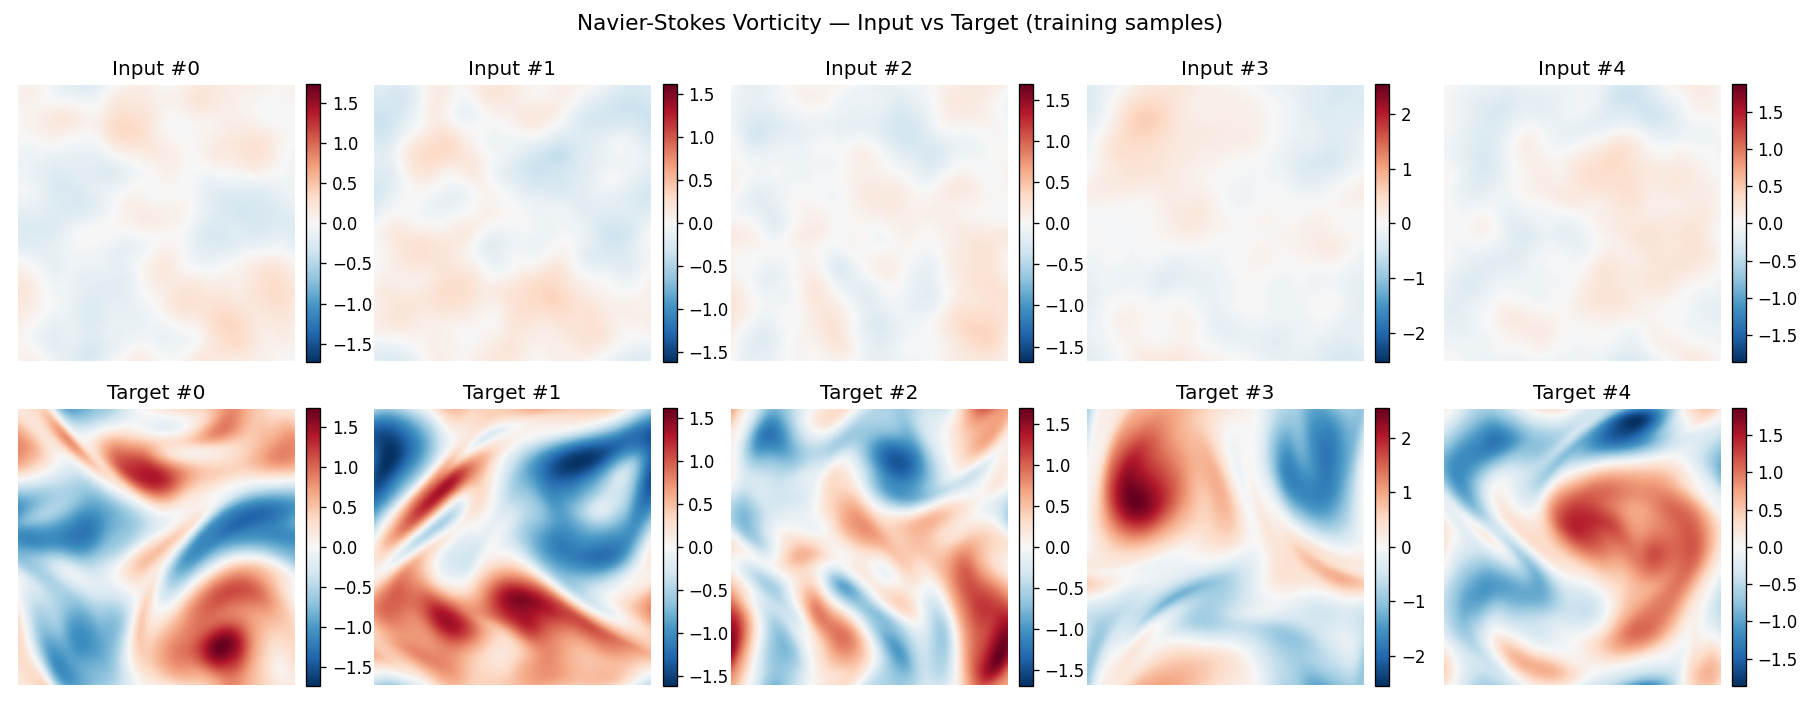
\includegraphics[width=\linewidth]{sample_pairs.png}
  \caption{Five input--target vorticity pairs from the training set.
           Top row: input $\omega(t)$ (smooth, low amplitude).
           Bottom row: target $\omega(t+1)$ (more turbulent, wider dynamic range).
           Color scale: RdBu\_r, red = positive/clockwise vorticity,
           blue = negative/counter-clockwise.}
  \label{fig:sample_pairs}
\end{figure}

% ─── METHODS ─────────────────────────────────────────────────────────────────
\section{Methods}
\label{sec:methods}

\subsection{FNO Architecture}

Our FNO2d implementation follows Li et al.\ \cite{li2021fno} closely.
The input vorticity field (1 channel) is augmented with a 2D coordinate grid
($gx$, $gy$) to produce a 3-channel input, then lifted to a 64-channel feature
map via a learned 1$\times$1 convolution.
Four Fourier blocks follow, each performing a spectral convolution (truncated to
12 Fourier modes per spatial dimension) summed with a bypass 1$\times$1
convolution, followed by GELU activation.
The output is projected from 64 channels to 128, then to 1, via two further
1$\times$1 convolutions with a GELU in between.
Total parameters: \textbf{4.7M}.

\subsection{U-Net Architecture}

Our U-Net uses a 4-level encoder--decoder structure.
The encoder doubles channels at each level (64$\to$128$\to$256$\to$512) while
halving spatial resolution via $2\times 2$ max-pooling.
The decoder uses bilinear upsampling and concatenates the corresponding encoder
feature map at each level.
Each block applies two 3$\times$3 convolutions with BatchNorm and ReLU.
Total parameters: \textbf{31M}.

\subsection{Training}

Both models are trained for 100 epochs on an NVIDIA GeForce RTX 2060 (6 GB
VRAM) with the following settings:
\begin{itemize}
  \item Loss: relative $L^2$ error,
        $\mathcal{L} = \|\hat{u} - u\|_2 / \|u\|_2$
  \item Optimizer: Adam, initial learning rate $10^{-3}$
  \item LR schedule: cosine annealing to $10^{-5}$
  \item Batch size: 20
\end{itemize}
Checkpoints are saved whenever validation loss improves.
Training is logged with MLflow.

% ─── RESULTS ─────────────────────────────────────────────────────────────────
\section{Results}
\label{sec:results}

\subsection{Standard Evaluation}

Table~\ref{tab:standard} reports test-set relative $L^2$ error, throughput, and
latency for both models.
FNO achieves roughly $3\times$ lower error than U-Net while using $6.6\times$
fewer parameters and running $2.2\times$ faster.

\begin{table}[t]
  \centering
  \caption{Standard evaluation on the 128$\times$128 test set.}
  \label{tab:standard}
  \begin{tabular}{lrrrr}
    \toprule
    Model  & Params & Rel-$L^2$$\downarrow$ & Throughput$\uparrow$ & Latency$\downarrow$ \\
           &        &                        & (samp/s)              & (ms/samp) \\
    \midrule
    FNO    & 4.7M   & \textbf{0.0348}        & \textbf{499.2}        & \textbf{2.003} \\
    U-Net  & 31M    & 0.1029                 & 227.0                 & 4.406 \\
    \bottomrule
  \end{tabular}
\end{table}

Figure~\ref{fig:predictions} shows side-by-side predictions from both models
on six test samples spanning the range of FNO error (best to median to worst).
FNO predictions closely match the ground truth in both large-scale structure and
fine vortex detail.
U-Net captures the broad structure but misses fine-grained vorticity features
and exhibits higher pointwise error throughout.

\begin{figure*}[tb]
  \centering
  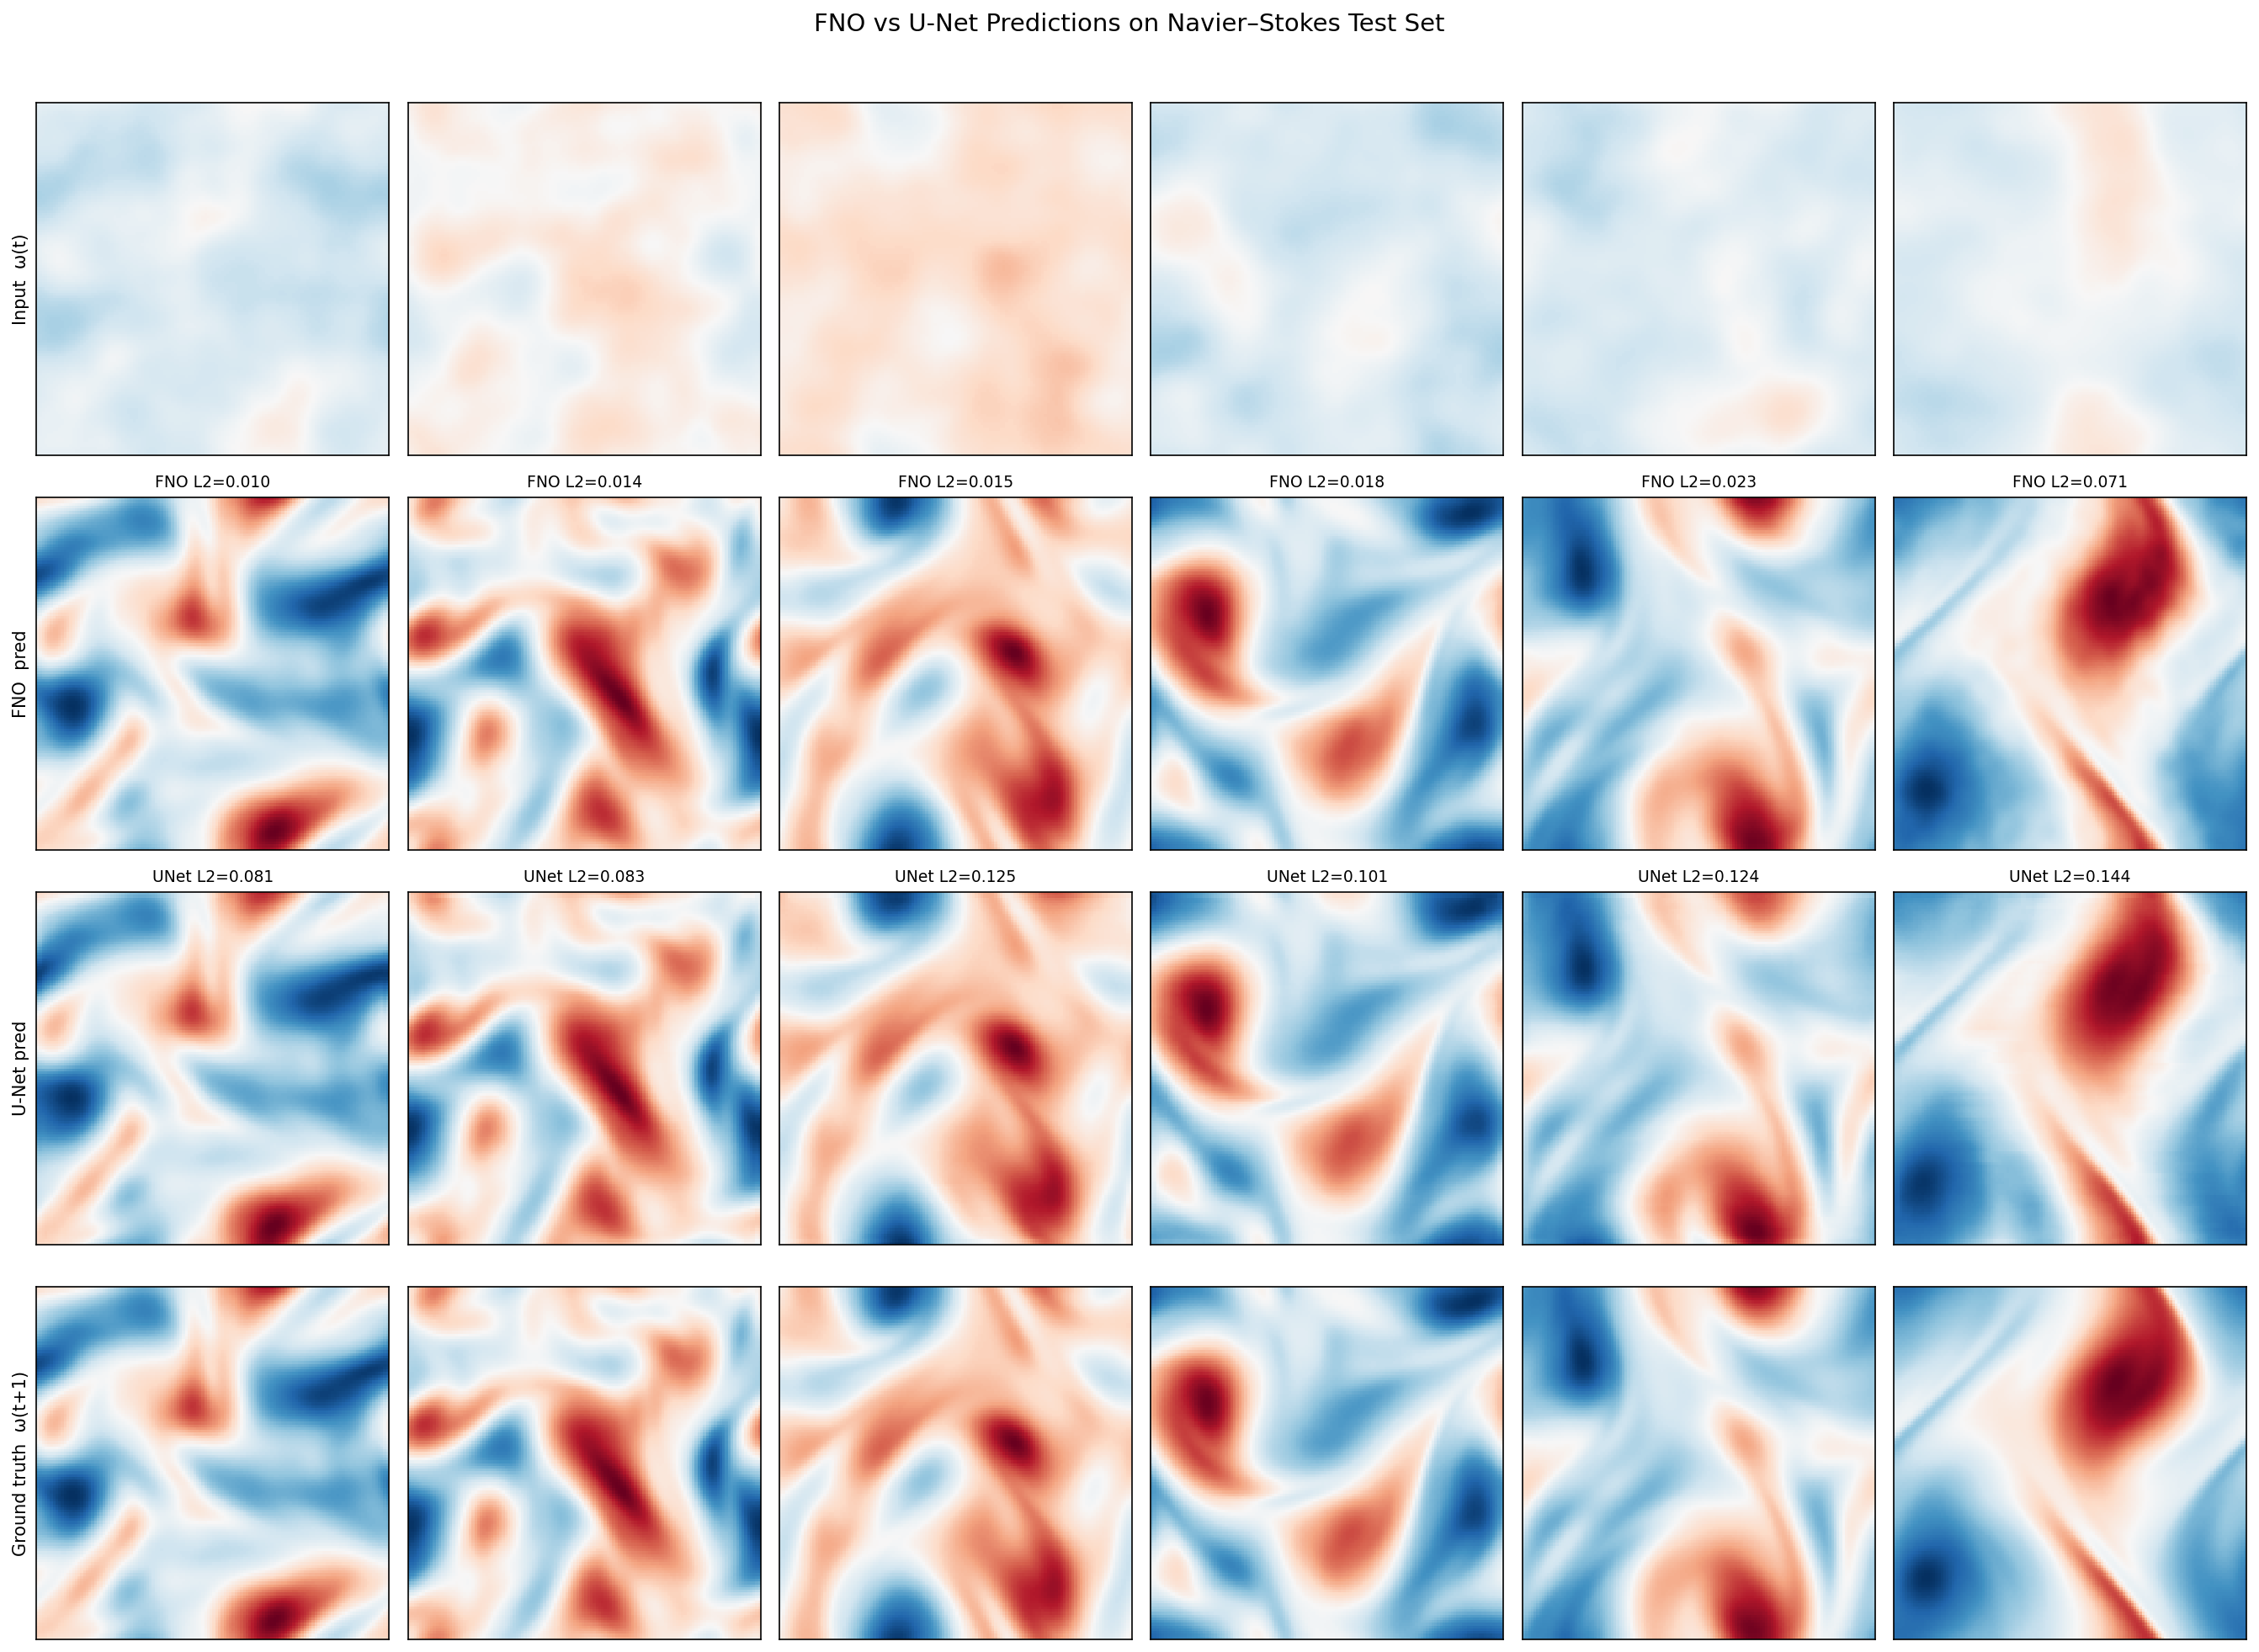
\includegraphics[width=\textwidth]{predictions.png}
  \caption{Six test samples ordered from lowest to highest FNO error.
           Rows: input $\omega(t)$ / FNO prediction / U-Net prediction / ground
           truth $\omega(t+1)$.
           Per-sample relative $L^2$ scores annotated per column.}
  \label{fig:predictions}
\end{figure*}

Figure~\ref{fig:error_maps} shows absolute error maps $|\hat{u} - u|$ for both
models.
FNO errors are small and diffuse; U-Net errors are concentrated at vortex cores
and high-gradient regions, consistent with difficulty learning fine-scale turbulent
features.

\begin{figure*}[tb]
  \centering
  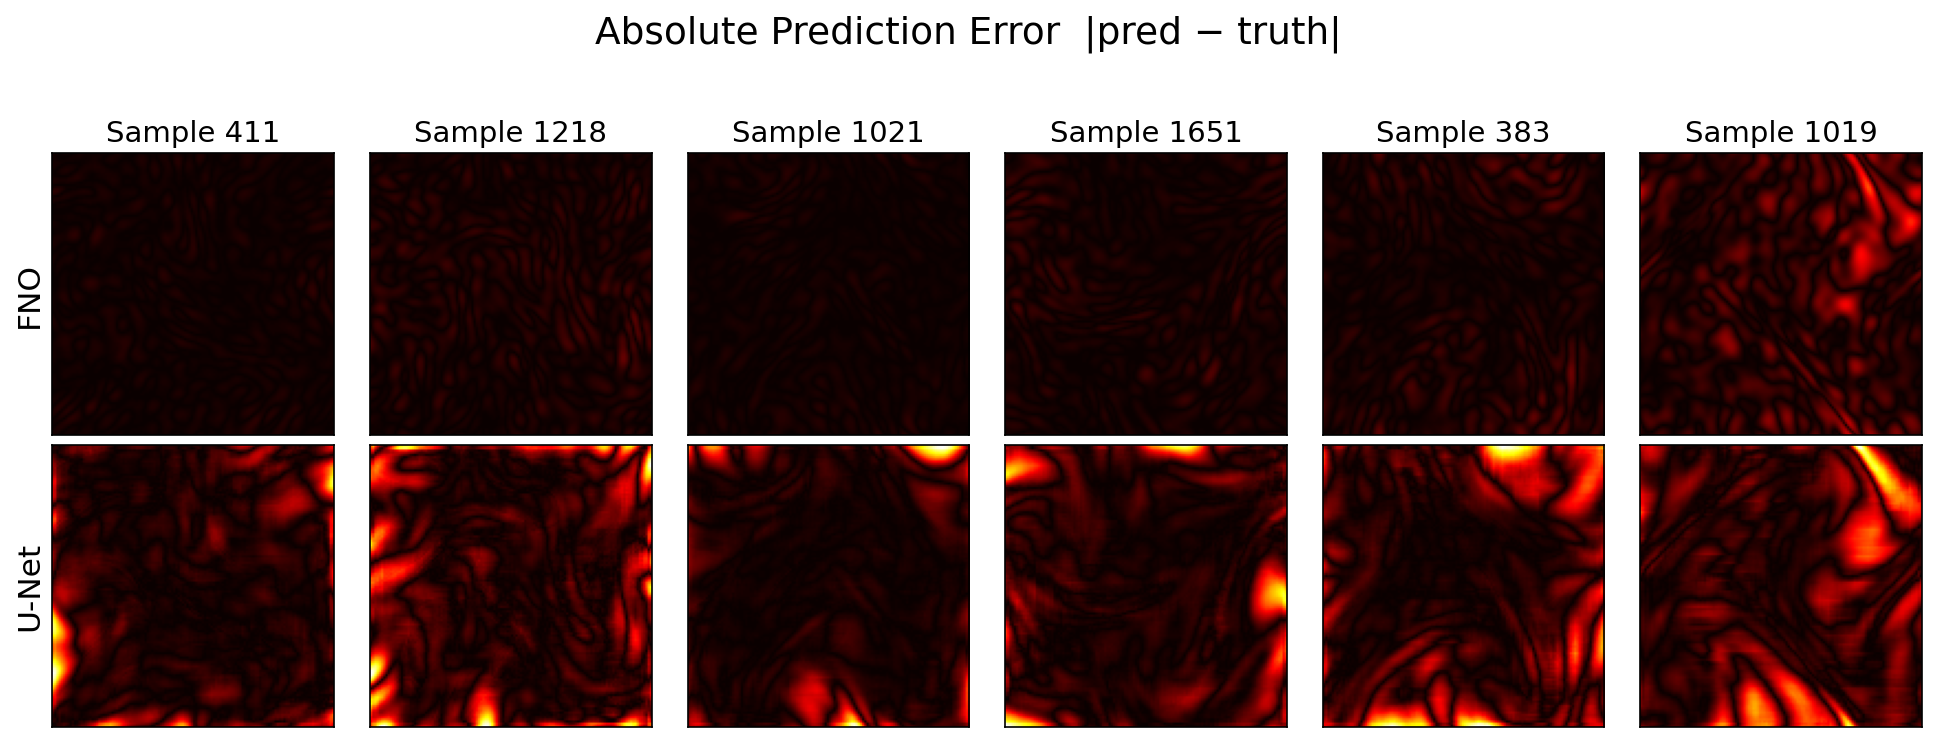
\includegraphics[width=\textwidth]{error_maps.png}
  \caption{Absolute prediction error $|\hat{u} - u|$ for FNO (top) and U-Net
           (bottom) on the same six samples as Figure~\ref{fig:predictions}.
           Color scale: hot (black = zero, white = maximum).
           U-Net errors are systematically larger and concentrated at vortex
           boundaries.}
  \label{fig:error_maps}
\end{figure*}

Figure~\ref{fig:error_hist} shows the per-sample relative $L^2$ distribution
across the full 2{,}000-sample test set.
FNO's distribution is narrow and concentrated near 0.035; U-Net's is broad and
shifted to the right, indicating consistently higher error with more variability.

\begin{figure}[t]
  \centering
  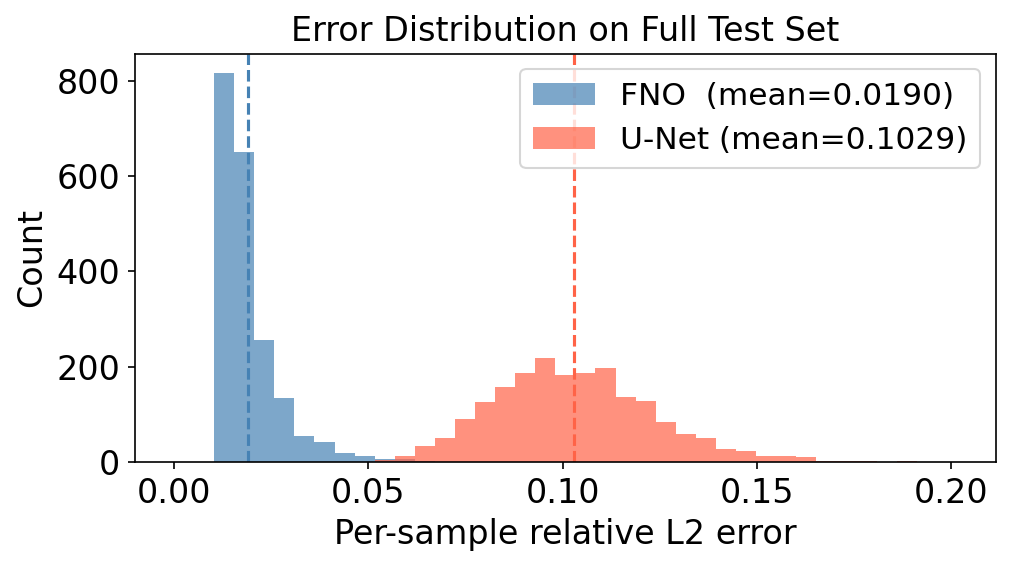
\includegraphics[width=\linewidth]{error_histogram.png}
  \caption{Distribution of per-sample relative $L^2$ error over the full test
           set.
           FNO (blue, mean $= 0.035$) is tightly concentrated; U-Net (red,
           mean $= 0.103$) is wider and skewed toward higher error.}
  \label{fig:error_hist}
\end{figure}

\subsection{Zero-Shot Super-Resolution}

Table~\ref{tab:superres} and Figure~\ref{fig:super_res} show results when both
models---trained only at 128$\times$128---are evaluated at 64$\times$64 and
256$\times$256 without any fine-tuning.
Ground truth at each resolution is obtained by bilinearly resampling the 128
test targets.

\begin{table}[t]
  \centering
  \caption{Zero-shot super-resolution: relative $L^2$ at unseen resolutions.}
  \label{tab:superres}
  \begin{tabular}{lcc}
    \toprule
    Resolution          & FNO Rel-$L^2$ & U-Net Rel-$L^2$ \\
    \midrule
    64$\times$64        & \textbf{0.0185}        & 0.4764 \\
    128$\times$128~(train) & \textbf{0.0190}     & 0.1029 \\
    256$\times$256      & \textbf{0.0188}        & 0.5941 \\
    \bottomrule
  \end{tabular}
\end{table}

FNO's error is essentially flat across all three resolutions, confirming that the
Fourier layers learn a resolution-invariant operator.
U-Net's error at 64$\times$64 and 256$\times$256 is $4.6$--$5.8\times$ higher
than at its training resolution, demonstrating that fixed spatial kernels do not
generalize across grid spacings.

\begin{figure}[t]
  \centering
  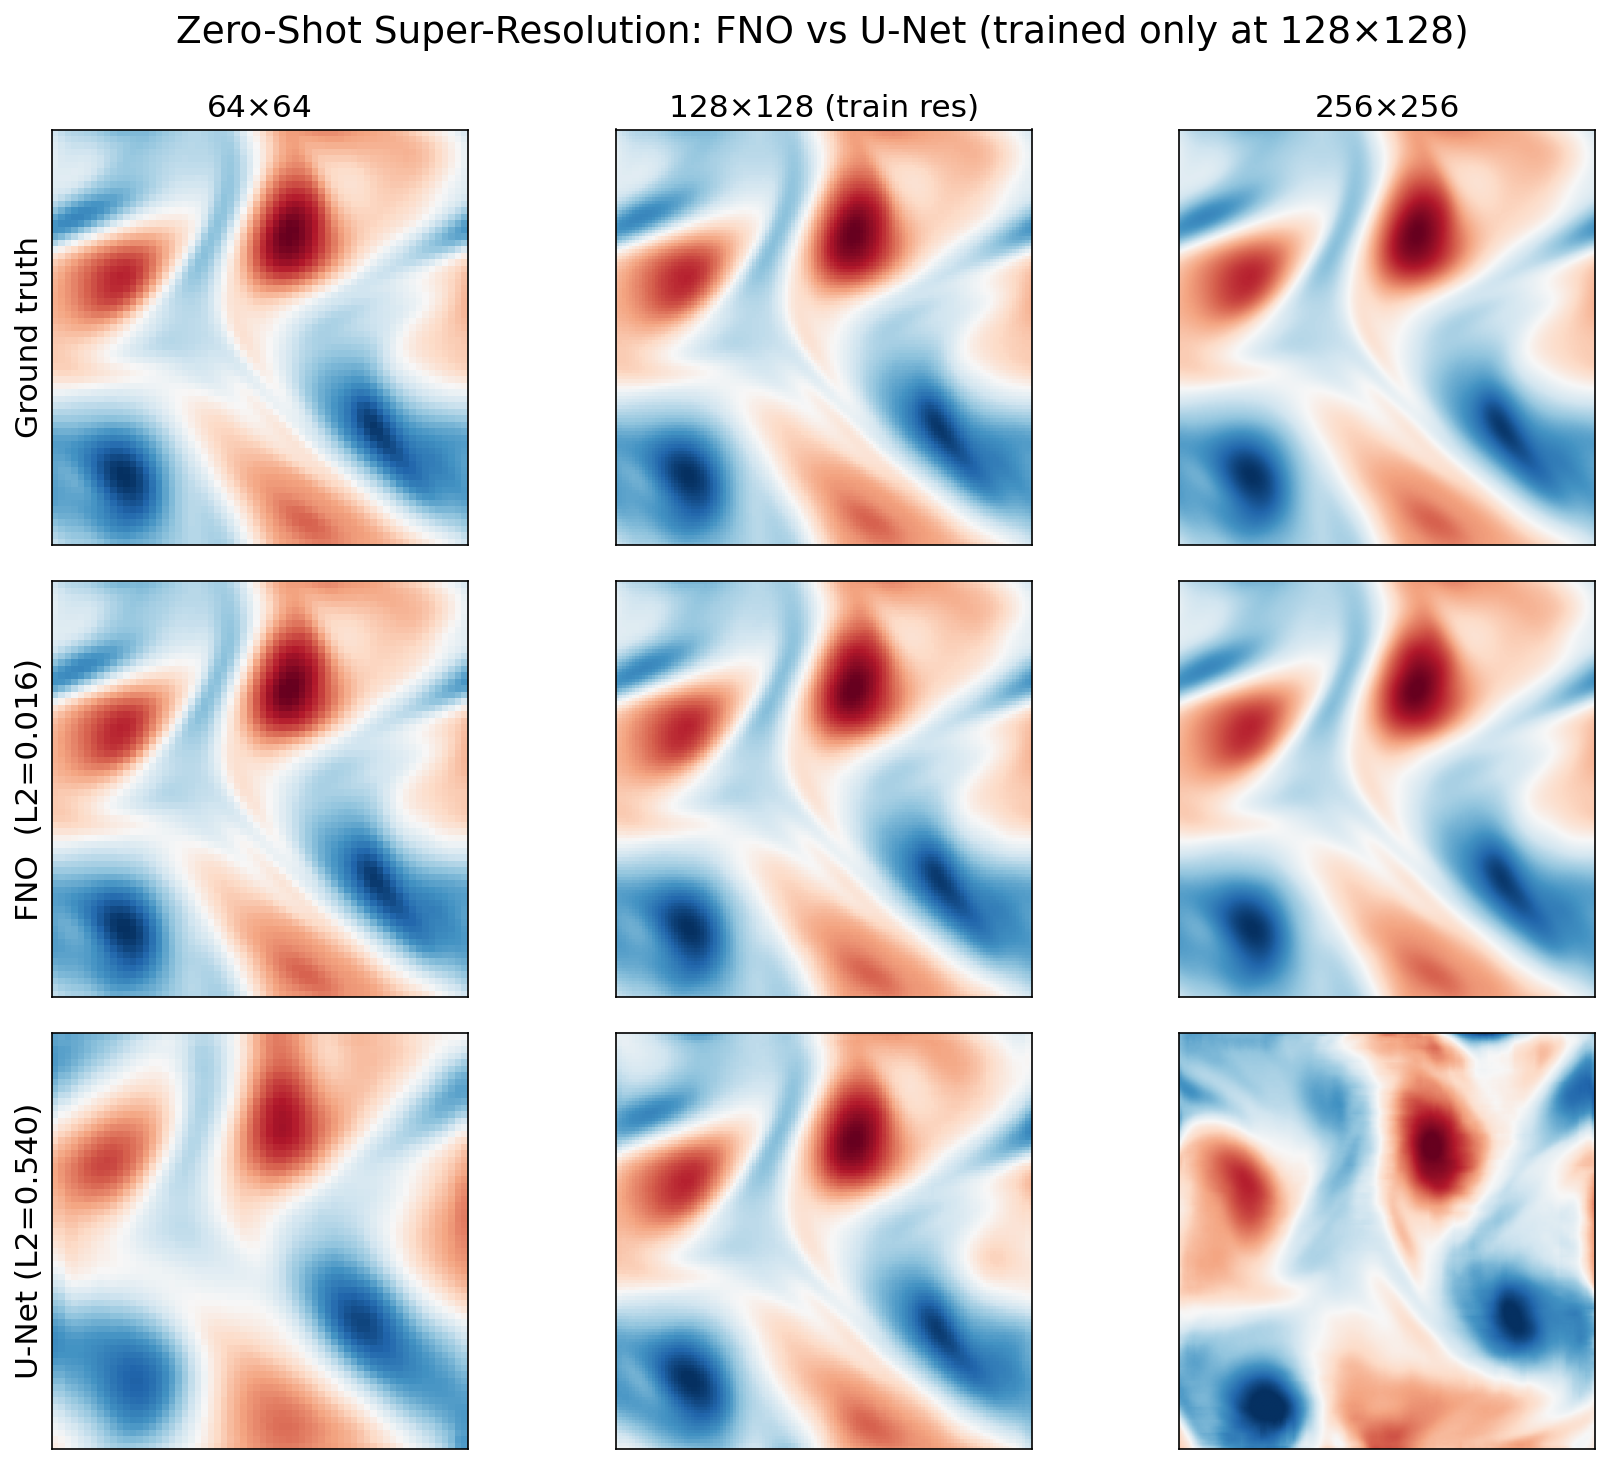
\includegraphics[width=\linewidth]{super_res.png}
  \caption{Zero-shot super-resolution on a single test sample.
           Columns: 64$\times$64, 128$\times$128 (train resolution), 256$\times$256.
           Rows: ground truth / FNO prediction / U-Net prediction.
           FNO maintains consistent visual quality at all resolutions.
           U-Net produces smooth but blurry outputs at 64$\times$64 and
           introduces artifacts at 256$\times$256.}
  \label{fig:super_res}
\end{figure}

% ─── DISCUSSION ──────────────────────────────────────────────────────────────
\section{Discussion}
\label{sec:discussion}

\paragraph{Why FNO outperforms U-Net.}
The performance gap stems from an inductive bias alignment.
The Navier--Stokes operator is global in nature: a vortex anywhere in the domain
can influence the flow everywhere else through the pressure field.
FNO captures this via global Fourier modes; U-Net's local $3\times 3$ kernels
must compose many layers to propagate information across the domain.
Additionally, the FFT-based parameterization of FNO directly represents the
low-frequency energy content of the vorticity field, which dominates NS dynamics.

\paragraph{Resolution invariance.}
FNO's flat super-resolution curve is a direct consequence of Fourier convolutions
operating in frequency space: the learned weights multiply specific Fourier
coefficients, which carry the same physical meaning regardless of how many spatial
grid points discretize the domain.
The U-Net's degradation at unseen resolutions is expected: 3$\times$3 kernels at
128$\times$128 correspond to a specific physical length scale, which changes when
the grid spacing changes.

\paragraph{Parameter efficiency.}
Despite having 6.6$\times$ fewer parameters, FNO outperforms U-Net substantially.
This is consistent with the general finding that architecture-level inductive
biases can substitute for raw model capacity when the biases are well-matched to
the problem structure.

\paragraph{Limitations.}
Several limitations should be noted.
First, both models are trained and evaluated at a single fixed viscosity
$\nu = 10^{-4}$; generalization across viscosities or forcing functions is not
tested.
Second, we evaluate only single-step prediction; autoregressive rollout over many
timesteps is likely to accumulate error.
Third, the super-resolution ground truth is obtained by bilinear downsampling
of 128$\times$128 data, not from independent high-resolution simulations, so the
256$\times$256 evaluation is a proxy.

% ─── CONCLUSION ──────────────────────────────────────────────────────────────
\section{Conclusion}
\label{sec:conclusion}

We trained and evaluated a Fourier Neural Operator and a U-Net on 2D
Kolmogorov-forced Navier--Stokes time-stepping.
FNO achieves $3\times$ lower relative $L^2$ error with $6.6\times$ fewer
parameters and $2.2\times$ higher inference throughput.
In zero-shot super-resolution, FNO's error remains flat while U-Net's degrades
by up to $5.8\times$.

These results support the conclusion that neural operators, which encode physical
structure---specifically, the frequency-space nature of PDE operators---directly
into the architecture, outperform generic convolutional baselines on PDE surrogate
modelling tasks.
The FNO framework represents a principled step toward fast, data-efficient neural
simulators that can generalize across discretizations.

% ─── REFERENCES ──────────────────────────────────────────────────────────────
\bibliographystyle{ACM-Reference-Format}
\bibliography{refs}

\end{document}
